\documentclass[border=10pt]{standalone}
\usepackage[svgnames]{xcolor}
\usepackage{amsmath}
\usepackage{pgfplots}
\pgfplotsset{compat=newest}
\usepackage[sfdefault]{FiraSans}
\usepackage{FiraMono}
\renewcommand*\familydefault{\sfdefault}
\begin{document}
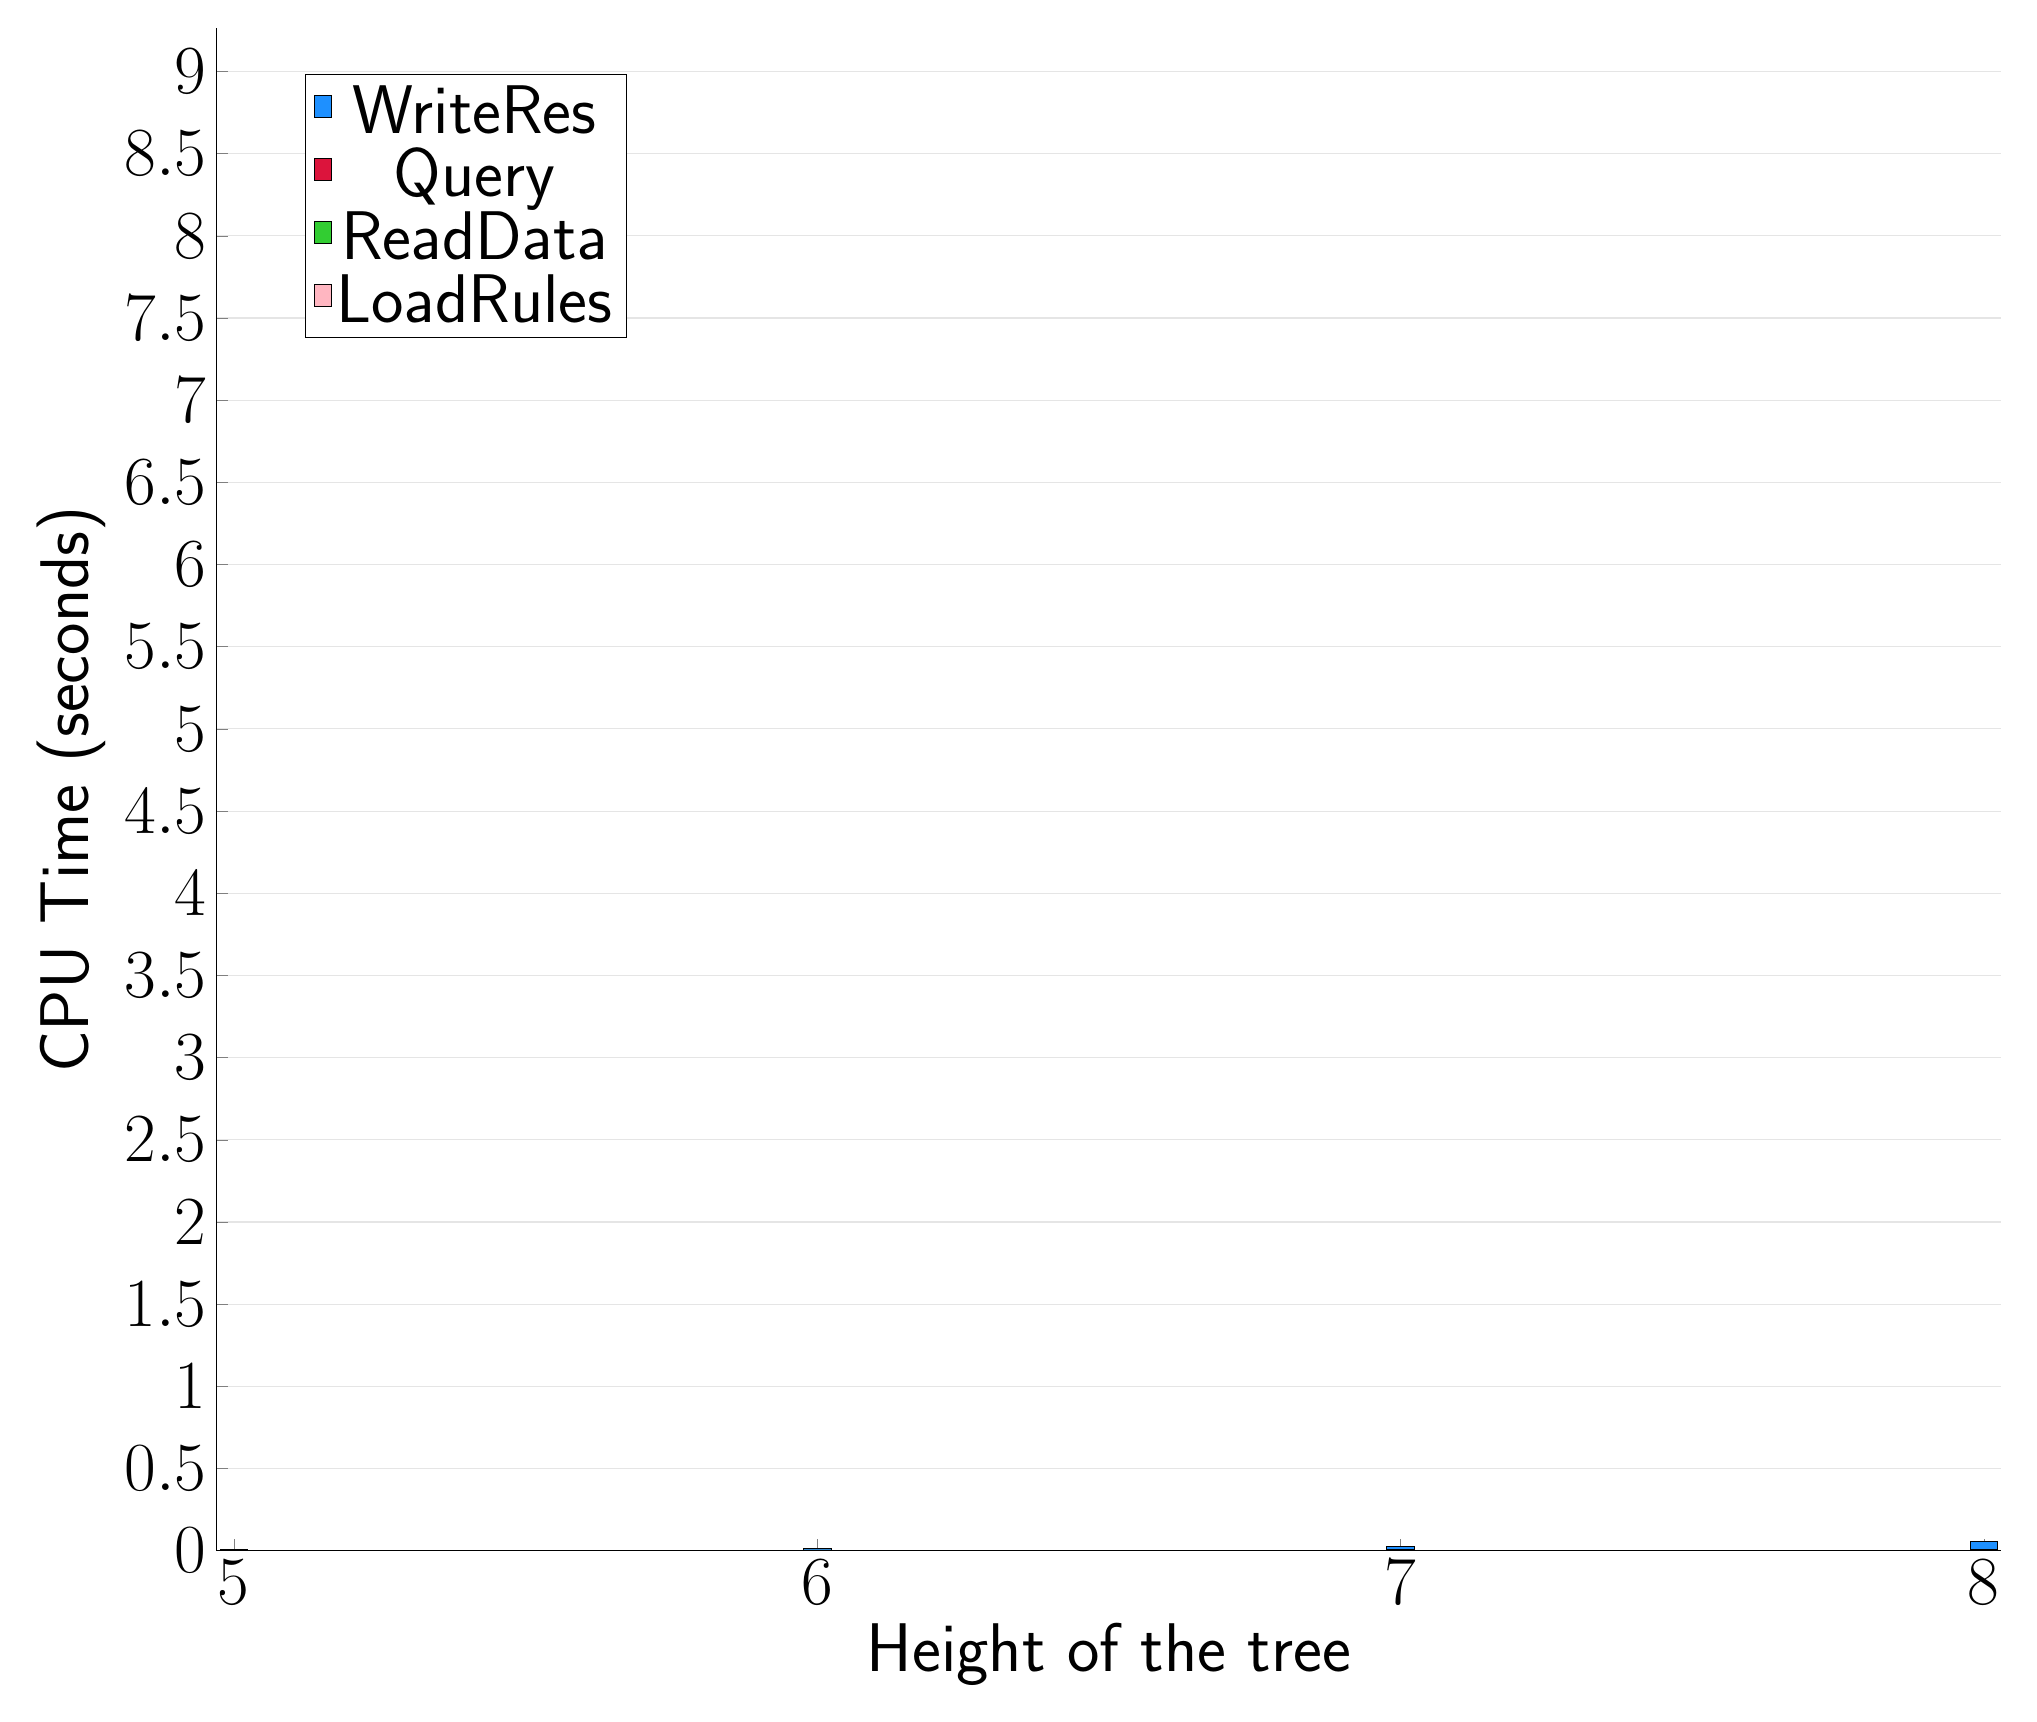
\begin{tikzpicture}
\begin{axis}[
   ybar stacked,
   width=2\textwidth,
   bar width=0.35cm,
   ymajorgrids, tick align=inside,
   major grid style={draw=gray!20},
   xtick=data,
   ymin=0, ymax=9.263333335518837,
   axis x line*=bottom,
   axis y line*=left,
   enlarge x limits=0.01,
   legend style={
       at={(0.23, 0.97)},
       anchor=north east,
       legend columns=1,
       font=\Huge,
   },
   ylabel={CPU Time (seconds)},
   xlabel={Height of the tree},
   label style={font=\Huge},
   tick label style={font=\Huge},
]
\addlegendimage{fill=DodgerBlue, draw=black, line width=0.2pt}
\addlegendentry{WriteRes}
\addlegendimage{fill=Crimson, draw=black, line width=0.2pt}
\addlegendentry{Query}
\addlegendimage{fill=LimeGreen, draw=black, line width=0.2pt}
\addlegendentry{ReadData}
\addlegendimage{fill=LightPink, draw=black, line width=0.2pt}
\addlegendentry{LoadRules}
\addplot +[fill=LightPink, draw=black, line width=0.2pt] coordinates {
(5, 0.0027089999999999966)
(6, 0.0031123333333333333)
(7, 0.003565)
(7, 0.003198666666666667)
(7, 0.0032556666666666667)
(8, 0.0029706666666666666)
(8, 0.0035943333333333335)
(8, 0.0022596666666666668)
};
\addplot +[fill=LimeGreen, draw=black, line width=0.2pt] coordinates {
(5, 0.000900333333333332)
(6, 0.001333)
(7, 0.002190000000000003)
(7, 0.001982666666666667)
(7, 0.0020286666666666634)
(8, 0.0035123333333333304)
(8, 0.0035373333333333333)
(8, 0.0022686666666666667)
};
\addplot +[fill=Crimson, draw=black, line width=0.2pt] coordinates {
(5, 3.0333333333335932e-05)
(6, 5.933333333333254e-05)
(7, 0.00014433333333333168)
(7, 0.00012666666666666593)
(7, 0.00012800000000000298)
(8, 0.000317333333333334)
(8, 0.0003413333333333347)
(8, 0.00022400000000000198)
};
\addplot +[fill=DodgerBlue, draw=black, line width=0.2pt] coordinates {
(5, 0.002318666666666664)
(6, 0.009039666666666666)
(7, 0.021722)
(7, 0.021959333333333334)
(7, 0.02112133333333333)
(8, 0.05167966666666666)
(8, 0.04830466666666666)
(8, 0.05009933333333333)
};
\end{axis}
\end{tikzpicture}

\end{document}
